%iffalse
\let\negmedspace\undefined
\let\negthickspace\undefined
\documentclass[journal,12pt,onecolumn]{IEEEtran}
\usepackage{cite}
\usepackage{amsmath,amssymb,amsfonts,amsthm}
\usepackage{algorithmic}
\usepackage{multicol}
\usepackage{graphicx}
\usepackage{textcomp}
\usepackage{xcolor}
\usepackage{txfonts}
\usepackage{listings}
\usepackage{enumitem}
\usepackage{mathtools}
\usepackage{gensymb}
\usepackage{comment}
\usepackage[breaklinks=true]{hyperref}
\usepackage{tkz-euclide} 
\usepackage{listings}
\usepackage{gvv}                                        
%\def\inputGnumericTable{}                                 
\usepackage[latin1]{inputenc}                                
\usepackage{color}                                            
\usepackage{array}                                            
\usepackage{longtable}                                       
\usepackage{calc}                                             
\usepackage{multirow}                                         
\usepackage{hhline}                                           
\usepackage{ifthen}                                           
\usepackage{lscape}
\usepackage{tabularx}
\usepackage{array}
\usepackage{float}
\newtheorem{theorem}{Theorem}[section]
\newtheorem{problem}{Problem}
\newtheorem{proposition}{Proposition}[section]
\newtheorem{lemma}{Lemma}[section]
\newtheorem{corollary}[theorem]{Corollary}
\newtheorem{example}{Example}[section]
\newtheorem{definition}[problem]{Definition}
\newcommand{\BEQA}{\begin{eqnarray}}
\newcommand{\EEQA}{\end{eqnarray}}
\newcommand{\define}{\stackrel{\triangle}{=}}
\theoremstyle{remark}
\newtheorem{rem}{Remark}

% Marks the beginning of the document
\begin{document}
\bibliographystyle{IEEEtran}
\vspace{3cm}

\title{\textbf{NCERT 10.3.3.3.6}}
\author{EE24BTECH11032- John Bobby}
\maketitle
\bigskip
\textbf{Question:}\\
Five years from now on, the age of Jacob will be $3$ times that of his son. Five years ago, Jacob's age was $7$ times that of his son. What are their present ages?\\
\textbf{Solution:}\\
Given information can be interpreted as,
\begin{align}
    x - 3y = 10\\
    x - 7y = -30
\end{align}
Simplifying and using matrix notation,
\begin{align}
    \myvec{
        1 & -3\\
        1 & -7
    } \myvec{x \\ y}= \myvec{ 10 \\ -30}
\end{align}
The matrix $A$ can be decomposed into:
\begin{align}
    A = L \cdot U,
\end{align}
where:
\begin{align}
    L &= \myvec{1 & 0 \\ 1 & 1}, \\
    U &= \myvec{1 & -3 \\ 0 & -4}.
\end{align}
\newline
Factorization of LU:\newline
Given a matrix $ \mathbf{A} $ of size $ n \times n $, LU decomposition is performed row by row and column by column. The update equations are as follows: \\ 
\qquad 1. Start by initializing $ \mathbf{L} $ as the identity matrix $ \mathbf{L} = \mathbf{I} $ and $ \mathbf{U} $ as a copy of $ \mathbf{A} $.\\
\qquad 2. For each column $ j \geq k $, the entries of $ U $ in the $ k $-th row are updated as:
\begin{align}
U_{k,j} = A_{k,j} - \sum_{m=1}^{k-1} L_{k,m} \cdot U_{m,j}\quad \forall \quad j \geq k
\end{align}
3. For each row $ i > k $, the entries of $ L $ in the $ k $-th column are updated as:
\begin{align}
L_{i,k} = \frac{1}{U_{k,k}} \brak{ A_{i,k} - \sum_{m=1}^{k-1} L_{i,m} \cdot U_{m,k}} \quad \forall \quad i > k
\end{align}
The system $A\vec{x} = \vec{b}$ is transformed into $L \cdot U \cdot \vec{x} = \vec{b}$. Let $\vec{y}$ satisfy $L\vec{y} = \vec{b}$:
\begin{align}
    \myvec{1 & 0 \\ 1 & 1} \myvec{y_1 \\ y_2} = \myvec{10\\ -30}.
\end{align}
Using forward substitution:
\begin{align}
    y_1 &= 10 \\
    y_1 + y_2 &= -30\\
    y_2 &= -40
\end{align}
Thus:
\begin{align}
    \vec{y} = \myvec{10 \\ -40}.
\end{align}

Next, solve $U\vec{x} = \vec{y}$:
\begin{align}
    \myvec{1 & -3 \\ 0 & -4} \myvec{x \\ y} = \myvec{10\\ -40}.
\end{align}

Using back substitution:
\begin{align}
	-4y=-40\\
    y=10\\
    x-3y=10\\
    x=40\\
    \myvec{x \\ y}= \myvec{40 \\ 10}
\end{align}
is the solution of the given system of equations.
\begin{figure}[h!]
   \centering
   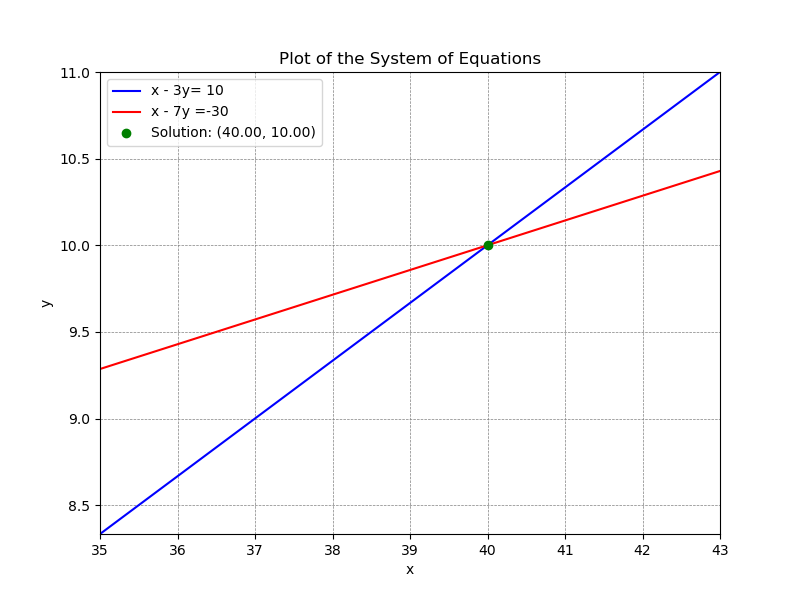
\includegraphics[width=1\columnwidth]{figs/Q6.png}
    \caption{Solution to set of linear equations}
\end{figure}
\end{document}

